\selectlanguage{italian}

\section{Modello di Yukawa}

Yukawa nel 1934 propose il primo modello per spiegare l'interazione tra nucleoni in termini di uno scambio di bosoni, ricalcando quello per l'interazione elettromagnetica.\\
In particolare, la teoria di campo proposta da Yukawa si basa sull'ipotesi che i nucleoni stessi siano le sorgenti del campo bosonico attraverso il quale interagiscono. Il campo d'interazione proposto deve avere le seguenti proprietà:
\begin{itemize}
	\item l'interazione deve avere un raggio d'azione $ a \sim 1\fm $;
	\item deve essere indipendente dalla carica elettrica (simmetria d'isospin);
	\item deve dipendere dallo stato di spin del sistema di nucleoni.
\end{itemize}
La terza condizione non era inclusa nel modello originale di Yukawa, e per semplicità si considera un potenziale a simmetria sferica. In questo caso, il campo bosonico può essere descritto dall'equazione di Klein-Gordon, che nel limite statico a simmetria sferica diventa:
\begin{equation*}
	\frac{1}{r^2} \frac{d}{dr} \left( r^2 \frac{d\phi(r)}{dr} \right) - \frac{mc}{\hbar} \phi(r) = 0
	\quad \Rightarrow \quad
	\phi(r) = \frac{\mathcal{N}}{r} e^{- r / a}\,,\,\, a = \frac{\hbar}{mc}
\end{equation*}
Si trova quindi che il campo di Yukawa, centrato in ciascun nucleone, è:
\begin{equation}
	V_{\text{Y}}(r) = \frac{g_s}{r} e^{-r / a}\,,\quad a = \frac{\hbar}{mc}
	\label{eq:9.1}
\end{equation}
dove $ g_s $ è la coupling constant dell'interazione. Dato che il raggio d'azione dell'interazione tra nucleoni è $ a \sim 1\fm $, si trova che il bosone mediatore, detto \textit{mesone} ($ \virgolette{stato intermedio} $) deve avere massa $ m \sim 200\mev/c^2 $: questo è in accordo col principio d'indeterminazione di Heisenberg, poiché detto $ \Delta t $ il tempo d'esistenza del mesone, si ha $ a = c \Delta t \sim \frac{\hbar c}{\Delta E} = \frac{\hbar}{mc} $.\\
Ad oggi, in realtà, è noto che il mesone di Yukawa non è una particella elementare, bensì composta da una coppia quark-antiquark: in particolare, l'interazione tra nucleoni a lunga distanza è mediata da mesoni $ \pi $ ($ 140\gev/c^2 $), a distanza ottimale ($ \approx 0.8\fm $) da mesoni $ \sigma $ ($ 500\mev/c^2 $) e a corta distanza, quando la forza diventa repulsiva, da mesoni $ \omega $ e $ \rho $ ($ 784\mev/c^2 $).\\
Inoltre, la teoria fondamentale alla base delle interazioni tra nucleoni è quella dell'interazione forte, la Cromodinamica Quantistica (QCD): questa descrive le interazioni tra quarks mediate da gluoni, non direttamente quelle tra nucleoni. Sebbene l'interazione tra nucleoni tramite scambio di mesoni sia ricavabile dalla QCD, essa va modificata quando avviene in presenza di altri nucleoni, come nel caso di un nucleo atomico: questo è un sistema quantistico a molti corpi estremamente complesso e per essere descritto richiede un modello d'interazione effettiva. Un tale esempio è la Lattice QCD, la quale può essere incorporata nella Chiral Effective Field Theory: questa teoria semplifica il modello del nucleo atomico considerando i nucleoni come gradi di libertà del sistema (al posto di quarks e gluoni).

\subsection{Simmetria di isospin}

Dato che il protone ed il neutrone non vengono distinti dall'interazione forte e che $ \left( m_n - m_p \right) / m_n \approx 10^{-3} $, Heisenberg propose di considerarli come due stati distinti di una stessa particella, il nucleone. In analogia allo spin, egli introdusse l'\textit{isospin} (o spin isotropico) $ I $, una grandezza adimensionale che si comporta matematicamente in maniera identica allo spin, assegnando $ I = \frac{1}{2} $ al nucleone e distinguendo protone e neutrone in base alla terza componente dell'isospin (analogo alla componente $ z $ dello spin): $ I_3 = +\frac{1}{2} $ per il protone e $ I_3 = -\frac{1}{2} $ per il neutrone.\\
L'hamiltoniana associata all'interazione forte è invariante per tutte le operazioni nello spazio astratto dell'isospin. Trascurando l'interazione elettromagnetica e quella debole, dunque, i livelli energetici del sistema sono degeneri e possono essere classificati secondo l'isospin totale $ I $: essendo analogo allo spin, i suoi possibili valori sono interi e semi-interi, e ad ogni suo valore corrisponde un multipletto di $ (2I + 1) $ autostati con la stessa energia ma con valori diversi di $ I_3 \in \left[ -I, I \right] $.\\
Mentre l'isospin totale si comporta come lo spin, la terza componente dell'isospin si comporta come la carica elettrica: mentre l'interazione forte, indipendente da $ I_3 $ e $ Q $ e dipendente solo da $ I $, conserva l'isospin totale, l'interazione elettromagnetica conserva solo $ I_3 $ e l'interazione debole non conserva l'isospin. L'indipendenza dell'interazione forte da $ I_3 $ e $ Q $ si può vedere, a livello nucleare, osservando che $ \ch{^7Li} $ e $ \ch{^7Be} $ hanno la stessa binding energy: questi sono \textit{mirror nuclei}, dunque hanno stesso spin e parità; formano inoltre un doppietto d'isospin con $ I = \frac{1}{2} $, dove $ \ch{^7Li} $ ha $ I_3 = -\frac{1}{2} $ e $ \ch{^7Be} $ ha $ I_3 = +\frac{1}{2} $. La simmetria di carica è verificata poiché ti trova che la forza protone-protone è uguale a quella neutrone-neutrone. Un'altra evidenza sperimentale deriva dalla seguente reazione:
\begin{equation*}
	\ch{^2H} + \ch{^2H} \rightarrow \ch{^4He} + \pi^0
\end{equation*}
L'isospin totale non è conservato, poiché $ 0 + 0 \neq 0 + 1 $, mentre $ I_3 $ lo è ($ 0 + 0 = 0 + 0 $), dunque la reazione è proibita dall'interazione forte ma amessa da quella elettromagnetica: sperimentalmente, si trova che la sezione d'urto della reazione è quella elettromagnetica e non quella forte, confermando l'ipotesi.\\
Anche i pioni formano un tripletto d'isospin: essi hanno proprietà identiche, eccetto la carica elettrica, e infatti per l'interazione forte essi sono come tre stati degeneri di una stessa particella. Dato che la degenerazione è di grado 3, il pione deve avere $ I = 1 $: $ \pi^+ $ ha $ I_3 = +1 $, $ \pi^0 $ ha $ I_3 = 0 $ e $ \pi^- $ ha $ I_3 = -1 $.\\
In generale, la relazione tra $ I_3 $, carica elettrica $ Q $ e numero barionico $ B \equiv \frac{1}{3} \left( n_q - n_{\bar{q}} \right) $ è dato dalla \textit{formula di Gell-Mann-Nishijima}:
\begin{equation}
	Q = I_3 + \frac{1}{2} B
	\label{eq:9.2}
\end{equation}
Questa formula considera solo quark di prima generazione ($ u,d $): nel caso si includano tutte le tre generazioni fermioniche, vanno aggiunti ulteriori termini.

\paragraph{Selection rules}

La conservazione dell'isospin porta a delle selection rules per i processi ad interazione forte. Ad esempio, si considerino le seguenti reazioni:
\begin{equation*}
	p + p \rightarrow \ch{^2H} + \pi^+
\end{equation*}
\begin{equation*}
	p + n \rightarrow \ch{^2H} + \pi^0
\end{equation*}
Entrambe hanno uno stato finale con $ I = 1 $; la prima reazione ha uno stato iniziale con $ I = 1 $, mentre la seconda ha uno stato iniziale che è una sovrapposizione di uno stato con $ I = 0 $ (50\%) ed uno con $ I = 1 $ (50\%): di conseguenza, dato che entrambe le reazioni sono dovute all'interazione forte, la prima procede interamente, mentre la seconda solo nel 50\% dei casi. Si deve quindi avere $ \sigma(pp \rightarrow d\pi^+) / \sigma(pn \rightarrow d\pi^0) = 2 $, che è proprio ciò che si osserva sperimentalmente.

\paragraph{Isospin dei quarks}

A partire da come sono costituiti $ p \left( uud \right) $ ed $ n \left( udd \right) $, si ha che i quarks $ u $ e $ d $ formano un doppietto di isospin $ I = \frac{1}{2} $, con $ I_3 = +\frac{1}{2} $ per $ u $ e $ I_3 = -\frac{1}{2} $ per $ d $. I rispettivi antiquarks hanno il segno di $ I_3 $ invertito, mentre gli altri quarks hanno $ I = 0 $.\\
Al giorno d'oggi si pensa che la simmetria di isospin sia dovuta alla quasi uguaglianza tra quark up e down ($ m_u \approx m_d $).

\subsection{Esperimenti di Conversi, Pancini e Piccioni}

Essendo nel giusto range di massa, inizialmente si pensò che il muone, allora noto come mesotrone, fosse il mesone di Yukawa (teorizzato nel 1934, mesotrone scoperto nel 1936). Con i loro esperimenti, però, Conversi, Pancini e Piccioni dimostrarono che questa identificazione era errata.\\
Il loro metodo sperimentale si basa sulle fast delayed coincidences, così da poter misurare con sufficiente precisione i tempi di decadimento dell'ordine dei microsecondi. L'apparato sperimentale permette di studiare la penetrazione e l'assorbimento di mesotroni cosmici in diversi materiali ed in base al loro segno: mesotroni negativi dovrebbero essere catturati nell'orbita idrogenoide K degli atomi e poi, se mediatori dell'interazione forte, interagire col nucleo atomico prima di decadere; mesotroni positivi, invece, dovrebbero essere respinti dal nucleo e decadere nello spazio vuoto tra gli atomi del materiale assorbitore.\\
Sperimentando con un assorbitore di grafite, nel 1946 CPP trovarono che i mesotroni positivi e negativi si comportavano in maniera praticamente identica e con vite medie troppo lunghe per essere effettivamente i mediatori dell'interazione forte: Fermi, Teller e Weisskopf calcolarono che la probabilità d'assorbimento di un mesotrone negativo in quiete è di un fattore $ 10^{12} $ inferiore a quella prevedibile per un mesone di Yukawa. Nel 1947 fu osservato il pione, che sarebbe poi stato identificato come il mesone di Yukawa.

\section{Mesoni}

I mesoni sono particelle composte da una coppia quark-antiquark: essi sono bosoni, poiché hanno spin intero. Mesoni liberi possono essere prodotti dalle collisioni tra nucleoni, decadendo rapidamente in mesoni più leggeri, fotoni o leptoni: i tempi di decadimento sono tipicamente $ 10^{-20} - 10^{-23}\,\text{s} $ per quelli forti, $ 10^{-16} - 10^{-18}\,\text{s} $ per quelli elettromagnetici e $ 10^{-8} - 10^{-10}\,\text{s} $ per quelli deboli.\\
I mesoni sono soggetti a tutte le interazioni fondamentali; inoltre, non esistono mesoni stabili.

\subsection{Pioni}

I mesoni $ \pi $ sono i mesoni più leggeri, responsabili per la maggior parte dei legami tra nucleoni. Essi possono avere carica elettrica $ \pm e $ o 0, dunque vengono indicati con $ \pi^{\pm} $ e $ \pi^0 $; inoltre, hanno isospin $ I = 1 $, con $ I_3 = \pm 1 $ per $ \pi^{\pm} $ ed $ I = 0 $ per $ \pi^0 $. I pioni carichi sono uno l'antiparticella dell'altro, mentre il pione neutro è l'antiparticella di sé stesso.

\subsubsection{Scoperta}

La scoperta del mesone $ \pi $ deriva dallo studio dei raggi cosmici secondari, in particolare utilizzando lastre fotografiche (metodo approntato da Powell): come si vede in Fig. \ref{pion-det}, in accordo con l'equazione di Bethe-Bloch (Eq. \ref{eq:3.5}), la ionizzazione del mezzo aumenta man mano che la particella rallenta (poiché perde più energia). In queste emulsioni, i pioni sono stati identificati da tracce di ionizzazione molto più dense di quelle degli elettroni.\\
I pioni così scoperti fittano molto bene nel modello di Yukawa: il potenziale risultante riproduce gli effetti osservati delle forze nucleari a grande distanza. Su scale comparabili alle dimensioni dei nucleoni, invece, bisogna considerare la struttura interna degli adroni (mesoni e barioni), e il modello a scambio di pioni risulta inadeguato. Gli effetti di spin-orbita e potenziale tensoriale che si manifestano a corto range sono modellati con scambio di mesoni $ \sigma $ e $ \omega,\rho $.

\begin{figure}
	\centering
	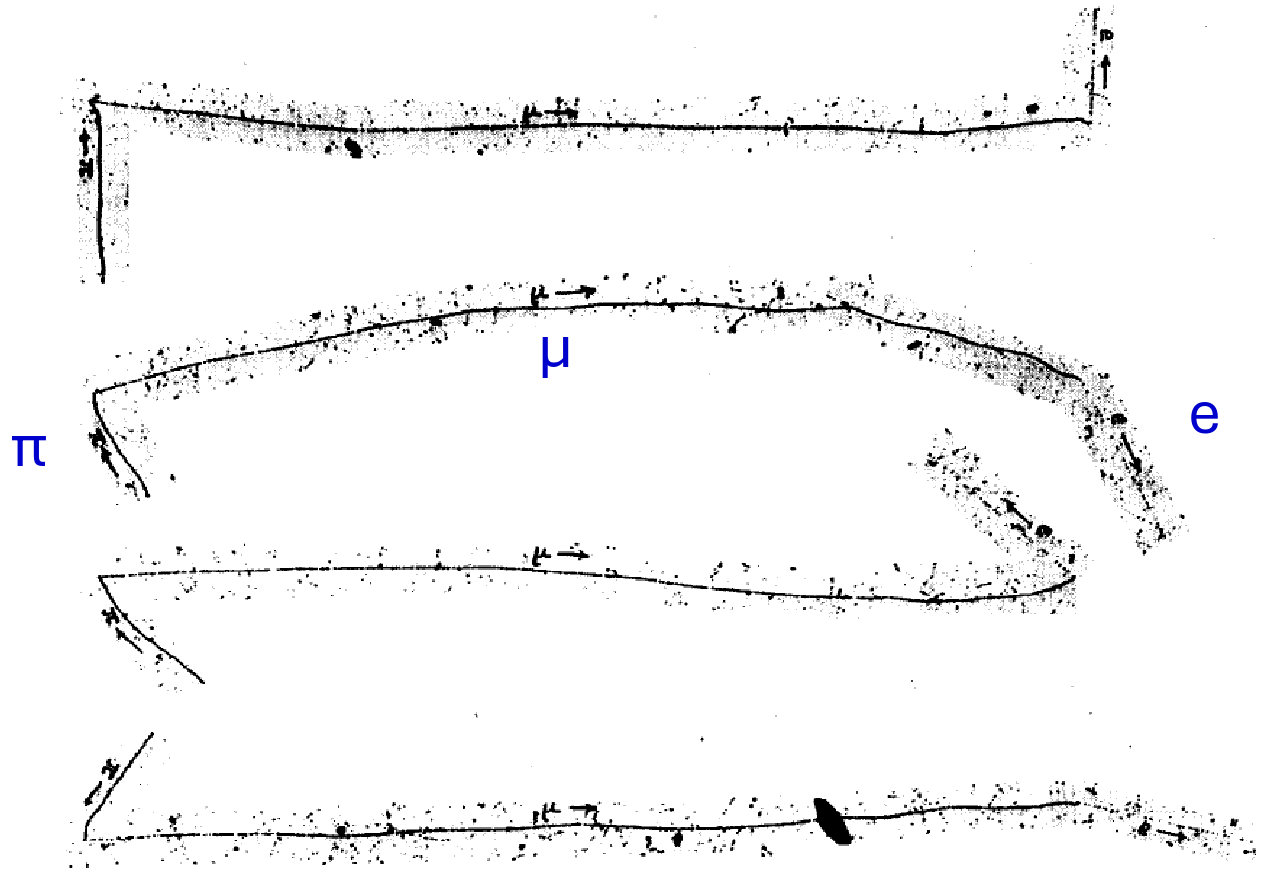
\includegraphics[width=0.70\textwidth]{pions.png}
	\caption{Emulsion of photographic plates showing pions decaying in muons, and then muons decaying in electrons.}
	\label{pion-det}
\end{figure}

\subsubsection{Massa}

La massa del pione negativo può essere determinata con molta precisione dall'energia dei raggi X emessi quando un $ \pi^- $ è catturato in un'orbita atomica e cade verso il nucleo, emettendo fotoni nel processo (analogamente a quelli emessi dalle transizioni di elettroni).\\
In particolare, l'apparato sperimentale utilizzato da Lu et al. produce pioni come particelle secondarie quando un fascio di protoni ad alta energia, proveniente da un sincrotrone, colpisce un target spesso. I pioni così prodotti vengono rallentati e stoppati nel materiale desiderato, dove i pioni negativi sono catturati in orbite atomiche e, decadendo di orbitale in orbitale (come stati eccitati), emettono fotoni. La differenza con gli elettroni è che i pioni si muovono molto più vicini al nucleo ($ r = \frac{4\pi \epsilon_0 h^2}{me^2} $, ma $ m_{\pi} \approx 270m_e $), dunque c'è una probabilità crescente per il processo di cattura $ \pi^- p \rightarrow n $: bisogna quindi studiare i raggi X da stati con $ n = 3,4,5 $, poiché il pione non sopravvive fino a quelli con $ n = 1,2 $. Per gli atomi di fosforo ($ Z = 15 $) e titanio ($ Z = 22 $) si trovano le transition energies $ \Delta E_{4\rightarrow3}(\ch{P}) = 40.49\kev $ e $ \Delta E_{5\rightarrow4}(\ch{Ti}) = 40.39\kev $, dunque dallo spettro energetico idrogenoide $ E_n = - \frac{m Z^2 e^4}{8 \epsilon_0^2 h^2} \frac{1}{n^2} $ si trova la massa del pione negativo $ m_{\pi^-} = 139.57\mev/c^2 $.\\
Questo metodo non si applica al pione positivo. Dallo studio del suo decadimento $ \pi^+ \rightarrow \mu^+\nu_{\mu} $ si trova $ m_{\pi^+} = 139.57\mev/c^2 $.\\
Per quanto riguarda la massa del pione neutro, essa può essere calcolata con la tecnica della massa invariante. La \textit{massa invariante} di un sistema è l'energia del sistema nel frame del centro di massa, che per un sistema di particelle è:
\begin{equation}
	\left( Mc^2 \right)^2 = \left( \sum E \right)^2 - \norm{\sum \ve{p} c}^2
	\label{eq:9.3}
\end{equation}
Per un sistema di due particelle, in unità naturali si trova:
\begin{equation*}
	M^2 = E_1^2 + E_2^2 + 2E_1 E_2 - p_1^2 - p_2^2 - 2\ve{p}_1 \cdot \ve{p}_2 = m_1^2 + m_2^2 + 2\left( E_1 E_2 - p_1 p_2 \cos \theta \right)
\end{equation*}
Nel caso in cui le masse a riposo delle particelle siano trascurabili, si ha:
\begin{equation*}
	M^2 = 2 E_1 E_2 \left( 1 - \cos \theta \right)
\end{equation*}
Questo è proprio il caso del decadimento $ \pi^0 \rightarrow \gamma\gamma $: plottando le misure di massa invariante per tutte le possibili coppie di fotoni, la distribuzione risulta avere un picco centrato in $ m_{\pi^0} $ con larghezza dipendente dalla risoluzione sperimentale e dalla decay width $ \Gamma \equiv \frac{\hbar}{\tau} $ ($ \sim 150\mev $ per decadimenti forti). In questo modo, si trova $ m_{\pi^0} = 134.97\mev/c^2 $.

\subsubsection{Decadimenti}

Essendo il mesone più leggero, il pione è la più leggera particella soggetta all'interazione forte: i suoi decadimenti sono dunque deboli o elettromagnetici, risultando in vite medie più lunghe rispetto agli altri mesoni.\\
In Fig. \ref{pion-det} è mostrato il principale decadimento dei pioni carichi, con branching ratio $ \approx 99.99 $\% e $ \tau = 2.6\cdot10^{-8}\,\text{s} $:
\begin{equation*}
	\pi^+ \rightarrow \mu^+ + \nu_{\mu}
\end{equation*}
con successivo decadimento $ \mu^+ \rightarrow e^+ \nu_e \bar{\nu}_{\mu} $.\\
Il pione neutro, invece, decade elettromagneticamente con branching ratio $ \approx 98.8 $\% e $ \tau = 0.8\cdot10^{-16}\,\text{s} $:
\begin{equation*}
	\pi^0 \rightarrow \gamma + \gamma
\end{equation*}
È possibile anche un Dalitz decay mode, con branching ratio $ \approx 1.2 $\%:
\begin{equation*}
	\pi^0 \rightarrow \gamma + e^+ + e^-
\end{equation*}

\subsubsection{Spin e parità}

Il fatto che il pione, in quanto mesone, debba avere spin intero è confermato dal decadimento $ \pi^0 \rightarrow \gamma \gamma $ e dalla reazione di produzione $ p p \rightarrow p n \pi^+ $.\\
Per studiare nel dettaglio lo spin del pione positivo, si sfruttano le due reazioni forti:
\begin{equation*}
	p + p \rightarrow d + \pi^+
	\qquad \qquad
	\pi^+ + d \rightarrow p + p
\end{equation*}
dove $ d $ indica il deuterone. L'interazione forte gode di simmetria per inversione temporale, a meno di un fattore cinematico: si parla di \textit{principio di bilancio dettagliato}, secondo il quale:
\begin{equation}
	\sigma \propto \frac{g}{k^2}
	\label{eq:9.4}
\end{equation}
dove $ p = \hbar k $ e $ g $ è un fattore statistico dipendente dallo spin. Per le reazioni considerate, si trova:
\begin{equation*}
	\frac{\sigma(pp \rightarrow d\pi^+)}{\sigma(d\pi^+ \rightarrow pp)} = \frac{g(pp \rightarrow d\pi^+)}{g(d\pi^+ \rightarrow pp)} \frac{k_{\pi^+}^2}{k_p^2} = \frac{(2s_{\pi^+} + 1)(2s_d + 1)}{\frac{1}{2} (2s_p + 1)^2} \frac{k_{\pi^+}^2}{k_p^2} = \frac{3}{2} \left( 2s_{\pi^+} + 1 \right) \frac{k_{\pi^+}^2}{k_p^2}
\end{equation*}
Si noti il fattore di $ \frac{1}{2} $ al denominatore, derivante dal principio d'esclusione che dimezza i possibili stati iniziali $ pp $. Confrontando i dati sperimantali con vari valori di $ s_{\pi^+} $, si trova che $ s_{\pi^+} = 0 $.\\
Per quanto riguarda il pione neutro, invece, si considera il decadimento $ \pi^0 \rightarrow \gamma \gamma $: nel rest frame di $ \pi^0 $, i due fotoni sono emessi in direzioni opposte; dato che $ s_{\gamma} = 1 $ e necessariamente si deve avere $ m_s = \pm 1 $ lungo la direzione del loro moto (dal fatto che le onde elettromagnetiche sono trasversali), si può avere $ s_{\pi^0} = 0,2 $: in analogia ai pioni carichi, si ha quindi $ s_{\pi^0} = 0 $.\\
La parità intrinseca del pione negativo può essere dedotta dalla seguente reazione:
\begin{equation*}
	\pi^- + d \rightarrow n + n
\end{equation*}
La parità iniziale è $ P_{\text{i}} = P_{\pi^-} P_d \left( -1 \right)^{\ell_{\text{i}}} $, dunque, selezionando $ \ell_{\text{i}} = 0 $ e ricordando che $ P_d = +1 $, si ha $ P_{\text{i}} = P_{\pi^-} $. Lo stato finale ha invece $ P_{\text{f}} = P_n P_n \left( -1 \right)^{\ell_{\text{f}}} = \left( -1 \right)^{\ell_{\text{f}}} $, dato che $ P_n = +1 $. Per lo stato iniziale si ha $ \ve{j}_{\text{i}} = \ve{s}_{\pi^-} + \ve{s}_d + \boldsymbol{\ell}_{\text{i}} $, ma $ s_{\pi^-} = 0 $, $ s_d = 1 $ e si è scelto $ \ell_{\text{i}} = 0 $, dunque $ j_{\text{i}} = 1 $. Per lo stato finale, invece, essendo i neutroni dei fermioni, la sua funzione d'onda totale deve essere antisimmetrica per scambio di neutroni: se la parte di spin della funzione d'onda è simmetrica ($ s_{n_1} + s_{n_2} = 1 $), la parte spaziale deve essere antisimmetrica ($ \ell_{\text{f}} $ dispari), mentre se $ s_{n_1} + s_{n_2} = 0 $ si deve avere $ \ell_{\text{f}} $ pari. La seconda opzione è esclusa dal fatto che $ j_{\text{i}} = 1 $, poiché se $ s_{n_1} + s_{n_2} = 0 $ l'unico modo per avere $ j_{\text{f}} = 1 $ è $ \ell_{\text{f}} = 1 $, che non è pari. L'unica opzione rimanente è che $ \ell_{\text{f}} $ sia dispari, il che implica $ P_{\pi^-} = -1 $.\\
Con un procedimento analogo si trova $ P_{\pi^+} = -1 $, considerando la reazione $ \pi^+ d \rightarrow p p $.\\
Per trovare $ P_{\pi^0} = -1 $, invece, si può studiare la polarizzazione degli elettroni nel decadimento $ \pi^0 \rightarrow e^+ e^+ e^- e^- $, oppure si può ricavarlo direttamente dalla reazione $ \pi^- d \rightarrow n n \pi^0 $.

\subsubsection{Produzione}

Le principali reazioni di produzione di pioni sono indotte dai raggi cosmici:
\begin{equation*}
	\begin{split}
		p + p
		&\rightarrow p + n + \pi^+ \\
		&\rightarrow p + p + \pi^0 \\
		&\rightarrow p + p + \pi^+ + \pi^-
	\end{split}
\end{equation*}
Queste reazioni possono essere riprodotte in acceleratori con frequenza anche maggiore, ma i raggi cosmici possono produrre energie maggiori. Si noti che viene rispettata la conservazione del numero barionico, poiché fermioni; per i mesoni, invece, in quanto bosoni, non vale nessuna legge di conservazione del numero, dunque le reazioni nucleone-nucleone possono produrre un numero arbitrario di mesoni, finché permesso dal bilancio energetico e dalla conservazione della carica.\\
Per le reazioni di produzione di due pioni, dall'Eq. \ref{eq:6.1} si trova la threshold energy $ T_{\text{th}} = 4m_{\pi} \approx 600\mev $, poiché $ Q = 2m_{\pi} $. Pioni vengono prodotti anche da raggi $ \gamma $ incidenti su nucleoni, secondo le reazioni:
\begin{equation*}
	\gamma + p \rightarrow n + \pi^+
	\qquad \qquad
	\gamma + p \rightarrow p + \pi^0
	\qquad \qquad
	\gamma + n \rightarrow p + \pi^0
\end{equation*}
Nelle cosiddette meson factories, si fanno incidere raggi $ \gamma $ su target solidi a basso $ Z $, producendo pioni con una threshold energy $ T_{\text{th}} \approx 150\mev $.

\subsubsection{Reazioni}

A partire da fasci di pioni prodotti in laboratorio, si possono studiare tre tipi di reazioni:
\begin{enumerate}
	\item scattering elastico: ad esempio $ \pi^+ + p \rightarrow p + \pi^+ $;
	\item scattering inelastico: ad esempio $ \pi^+ + p \rightarrow n + \pi^+ + \pi^+ $;
	\item scambio di carica: ad esempio $ \pi^- + p \rightarrow n + \pi^0 $;
\end{enumerate}
Studiando le reazioni $ \pi^{\pm} p $ si osservano delle grosse risonanze nelle cross-sections: si trova che queste risonanze pione-nucleone hanno energia, vita media, spin, parità e decay modes ben definiti, dunque sono delle strutture ben definite al pari di altre particelle come protoni e neutroni, sebbene estremamente short-lived.
In Fig. \ref{pion-scatt} si può notare la risonanza a $ T_{\pi} \approx 200\mev $, presente sia in $ \pi^+ p $ che in $ \pi^- p $ (sia per scattering elastico che per scambio di carica): questa risonanza, corrispondente ad una center-of-mass energy di $ 1232\mev $, è nota come risonanza $ \Delta(1232) $; le risonanze meno pronunciate sono risonanze $ N $.

\begin{figure}[!hb]
	\centering
	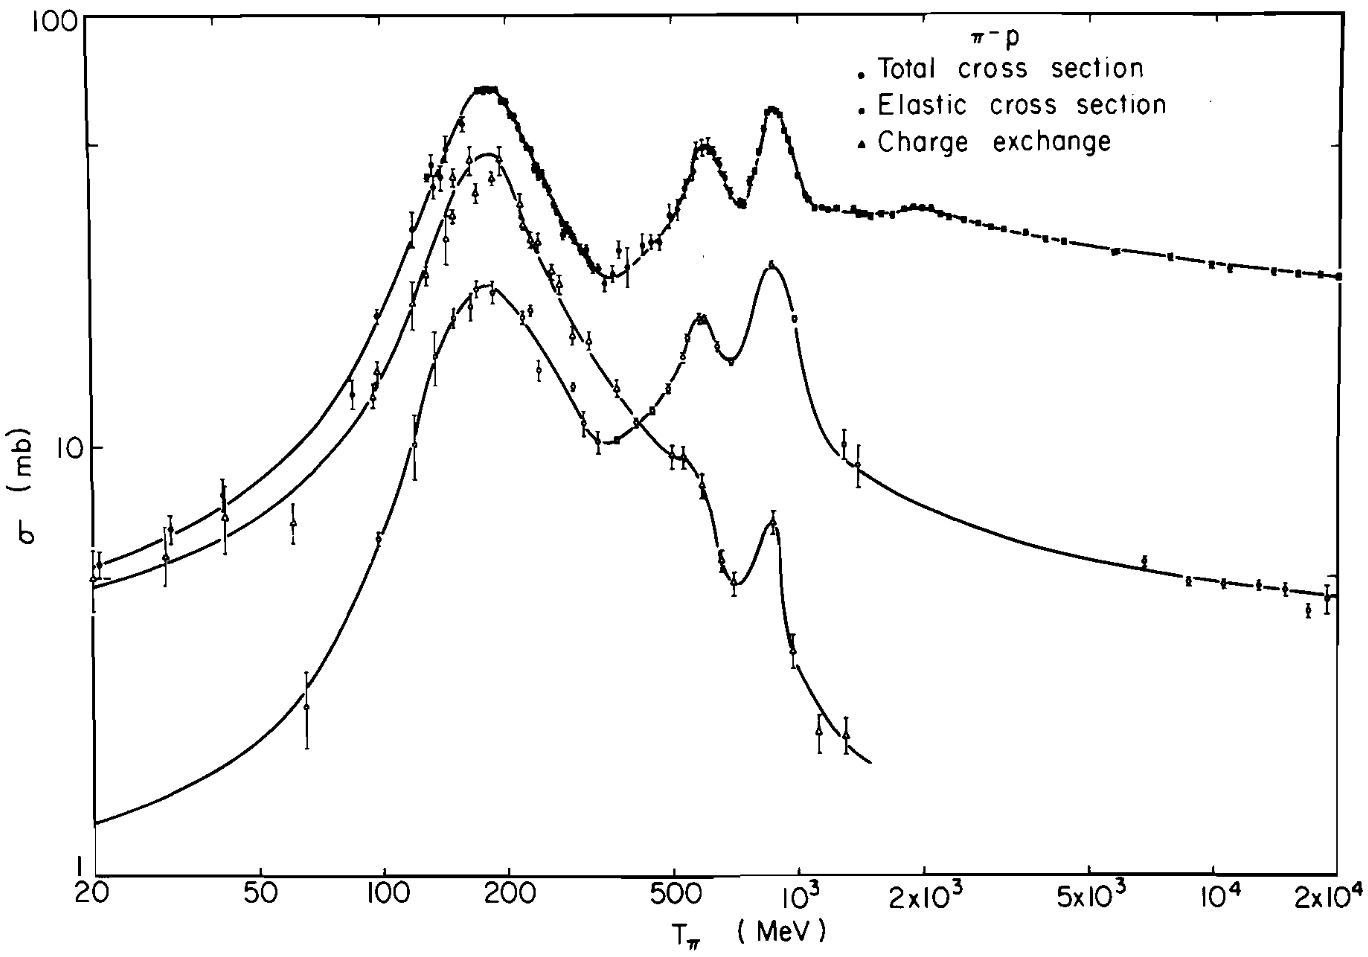
\includegraphics[width=0.70\textwidth]{pion-scatt.png}
	\caption{Cross-sections for $ \pi^- p $ reactions.}
	\label{pion-scatt}
\end{figure}

Le risonanze $ N $ e $ \Delta $ possono essere considerate come stati eccitati del nucleone: le risonanze $ \Delta $ esistono in quartetti di carica $ Q = +2,+1,0,-1 $, mentre le risonanze $ N $ in doppietti di carica $ Q = +1,0 $; a queste risonanze viene dunque assegnato un isospin $ I = \frac{3}{2} $ per le $ \Delta $ e $ I = \frac{1}{2} $ per le $ N $ (in accordo col coupling di nucleone con $ I = \frac{1}{2} $ e pione con $ I = 1 $). In assenza di interazioni elettromagnetiche, i membri di un multipletto avrebbero tutti la stessa massa: nella realtà, si osserva uno splitting di pochi MeV$ /c^2 $. Queste risonanze nucleoniche sono consistenti con quelle osservate in altri processi di scattering, come $ pp $, $ \gamma p $ e $ e^- p $.

\subsection{Risonanze}

Essendo i pioni i mesoni più leggeri, è possibile produrre mesoni più pesanti aumentando l'energia incidente nelle reazioni $ pp $ o $ \pi p $. Tutti i mesoni più pesanti del pione hanno masse superiori a $ 2m_{\pi} $, dunque, non essendoci leggi di conservazione sul numero mesonico, i loro decadimenti possono produrre due o più pioni tramite interazione forte, con $ \tau \sim 10^{-23}\,\text{s} $. Sebbene tali tempi di decadimento impediscano l'osservazione diretta, è possibile inferire l'esistenza di queste risonanze mesoniche dallo studio dei loro prodotti di decadimento: dalla distribuzione energetica di tali prodotti è possibile risalire alla decay width della risonanza, e dunque alla sua vita media.

\begin{figure}[!h]
	\centering
	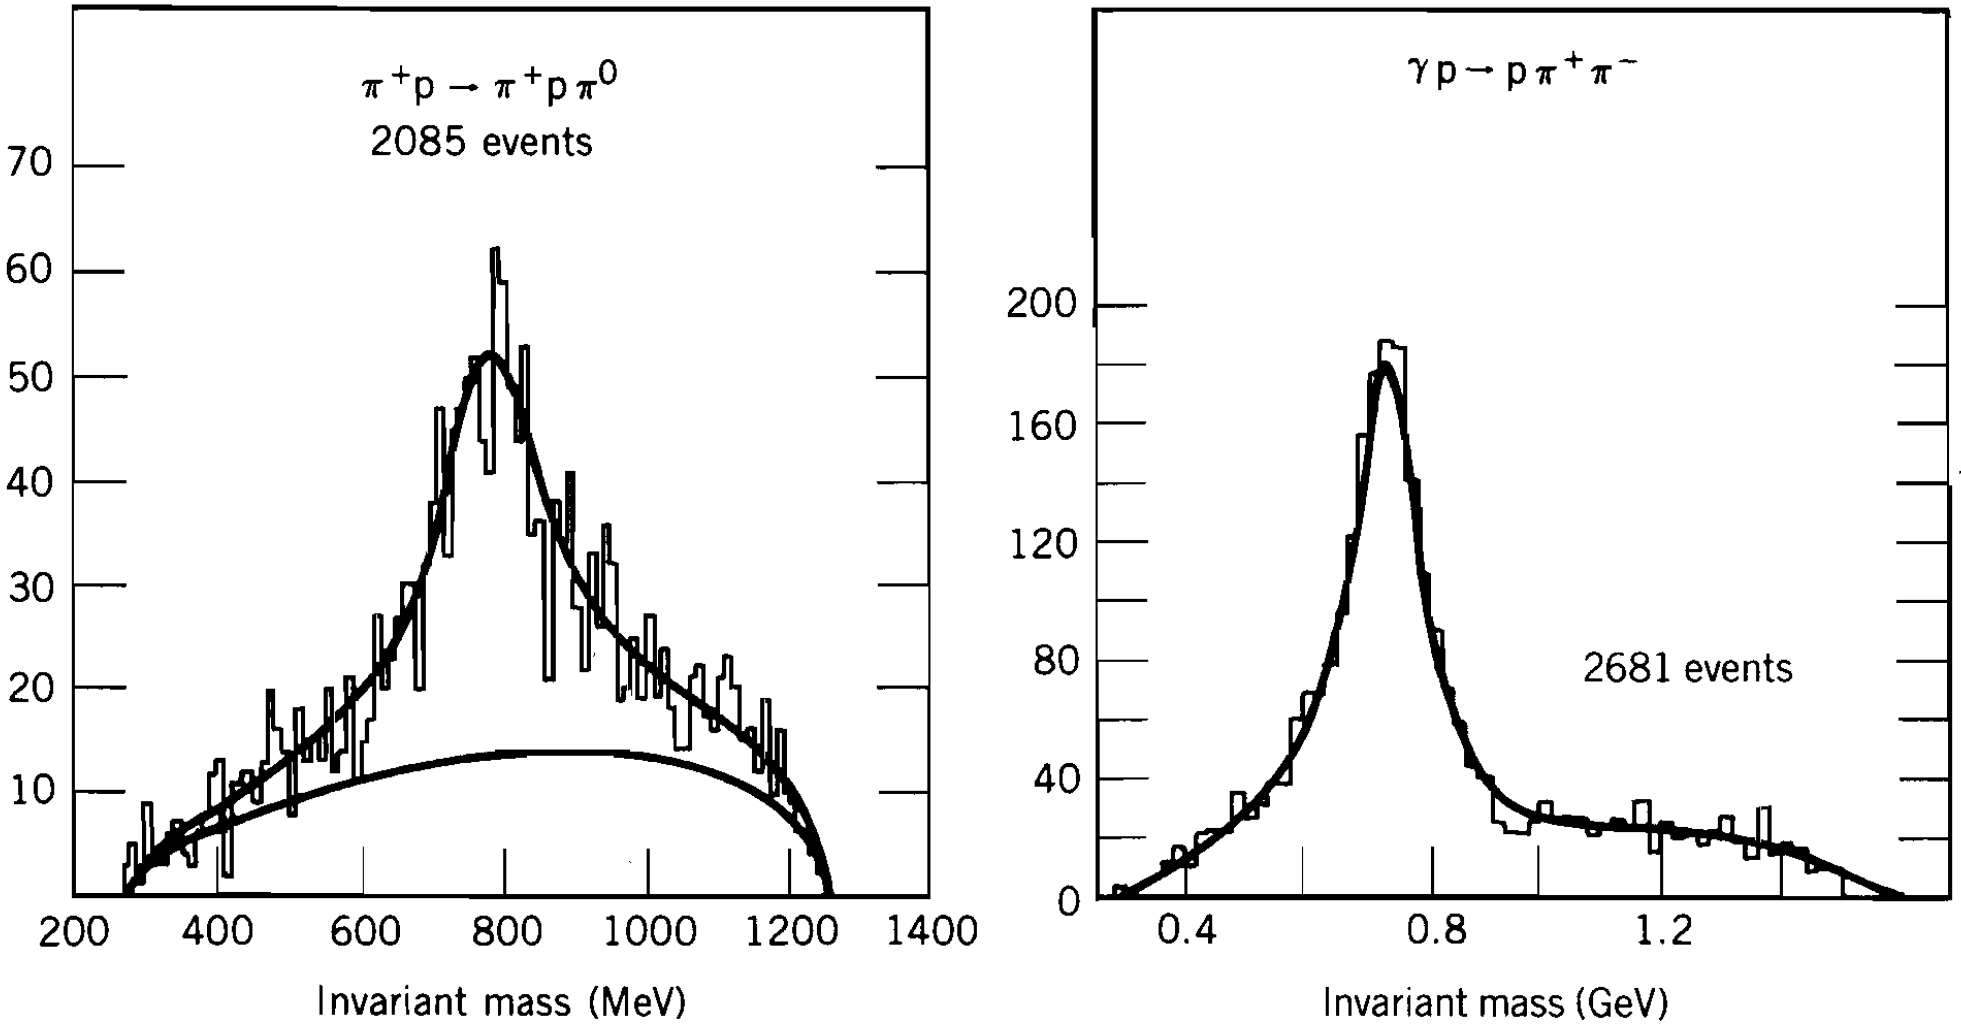
\includegraphics[width = 0.80\textwidth]{meson-reson.png}
	\caption{Invariant mass distribution for $ \pi^+ \pi^0 $ and $ \pi^+ \pi^- $, produced respectively by $ \pi^+ p \rightarrow p \pi^+ \pi^0 $ at $ 2.08\gev/c^2 $ incident momentum and $ \gamma p \rightarrow p \pi^+ \pi^- $ with $ E_{\gamma} = 2.8\gev $.}
	\label{meson-reson}
\end{figure}

In Fig. \ref{meson-reson} si possono vedere gli invariant mass plots per le reazioni $ \pi^+ p \rightarrow p \pi^+ \pi^0 $ e $ \gamma p \rightarrow p \pi^+ \pi^- $, nei quali è possibile identificare delle risonanze a circa $ 770\mev $, di larghezza $ 150\mev $ tipica dei decadimenti forti: questi sono identificabili come due mesoni, rispettivamente il mesone $ \rho^+ $ e quello $ \rho^0 $, i quali decadono in maniera forte come $ \rho^+ \rightarrow \pi^+ \pi^0 $ e $ \rho^0 \rightarrow \pi^+ \pi^- $.\\
Il mesone $ \rho $, così come il mesone $ \pi $, presenta un tripletto d'isospin $ I = 1 $: $ \rho^+ $ con $ I_3 = +1 $, $ \rho^0 $ con $ I_3 = 0 $ e $ \rho^- $ con $ I_3 = -1 $. Studiando i pioni prodotti dal decadimento, si trova che il mesone $ \rho $ ha spin $ s_{\rho} = 1 $ e parità $ P_{\rho} = -1 $.\\
Altre importanti risonanze mesoniche sono il mesone $ \omega $ a $ 783\mev $ e il mesone $ \eta $ a $ 549\mev $: il mesone $ \omega $ ha spin 1, isospin 0 e parità $ -1 $, mentre il mesone $ \eta $ spin 0, isospin 0 e parità $ -1 $, ed entrambi formano un singoletto elettricamente neutro. Il principale decay mode del mesone $ \omega $ è quello forte $ \omega \rightarrow \pi^+ \pi^- \pi^0 $, ma sono anche possibili quelli elettromagnetici $ \omega \rightarrow \pi^0 + \gamma $ e $ \omega \rightarrow \pi^+ \pi^- $ (non si conserva l'isospin): la decay width è $ \Gamma \approx 10\mev $, dunque la vita media del mesone $ \omega $ è circa un ordine di grandezza più lunga di quella del mesone $ \eta $. Il mesone $ \eta $, invece, decade principalmente in maniera elettromagnetica come $ \eta \rightarrow \gamma \gamma $, $ \eta \rightarrow \pi^0 \pi^0 \pi^0 $ ed $ \eta \rightarrow \pi^+ \pi^- \pi^0 $ (proibiti dalla conservazione dell'isospin): la decay width risultante è $ \Gamma \approx 0.8\kev $, corrispondente ad una vita media $ \tau \sim 10^{-18} \,\text{s} $, molto maggiore di quella dei mesoni $ \omega $ e $ \rho $ che decadono forte.\\
Infine, si deve tener conto che le risonanze mesoniche possono essere prodotte anche da collisioni $ e^+ e^- $ altamente energetiche, oltre che da quelle di particelle che interagiscono forte.

\subsection{Mesoni strani}

Negli anni '50 furono osservate delle particelle che, seppur prodotte da reazioni forti, decadevano con tempi lunghi caratteristici dei decadimenti deboli. Per questo motivo, furono chiamate particelle strane, e successivamente sarebbero state associate alla presenza di strange quarks nella loro composizione.
Alle particelle strane è associato un numero quantico di stranezza, il quale è conservato dalle interazioni forte ed elettromagnetica, mentre non lo è da quella debole.\\
La particella strana più leggera è il mesone $ K $, con massa di circa $ 500\mev/c^2 $, spin 0 e parità $ -1 $, e facente parte di un doppietto di isospin $ I = \frac{1}{2} $: $ K^+ $ con $ I_3 = \frac{1}{2} $ e $ K^0 $ con $ I_3 = -\frac{1}{2} $; le rispettive antiparticelle sono $ K^- $, con $ I_3 = -\frac{1}{2} $, e $ \bar{K}^0 $, con $ I_3 = \frac{1}{2} $. Similmente alla produzione di pioni, i kaoni possono essere prodotti da reazioni del tipo:
\begin{equation*}
	\pi^- + p \rightarrow n + K^- + K^+
\end{equation*}
Convenzionalmente si assegna stranezza $ S = +1 $ a $ K^+ $, dunque, essendo questa una reazione forte, si deve avere $ S = -1 $ per $ K^- $ per avere la conservazione della stranezza; inoltre, si trova $ S = +1 $ per $ K^0 $ ed $ S = -1 $ per $ \bar{K}^0 $. Una conseguenza del fatto che l'interazione forte conserva la stranezza è l'\textit{associated production}: le particelle strane sono sempre prodotte in coppie o set, mai sole, così da conservare la stranezza nulla iniziale. Essendo la particella strana più leggera, il kaone può decadere solo in particelle con stranezza nulla, quindi solo debolmente, risultando così in una vita media relativamente lunga $ \tau \sim 10^{-8}\,\text{s} $. I principali decay modes per il kaone positivo sono $ K^+ \rightarrow \mu^+ \nu_{\mu} $, $ K^+ \rightarrow \pi^+ \pi^0 $ e $ K^+ \rightarrow \pi^+ \pi^+ \pi^- $.\\
Ci sono molte risonanze mesoniche strane, le quali solitamente decadono in mesoni strani più leggeri senza violare la conservazione della stranezza. Un esempio è il mesone $ K^* $, risonanza a $ 892\mev $, il quale decade secondo $ K^* \rightarrow K \pi $: questo è un decadimento forte, ed infatti risulta $ \tau \sim 10^{-23}\,\text{s} $.

\section{Modello a quarks}

Per spiegare il particle zoo scoperto tra gli anni '50 e '60, fu proposto che tutti i mesoni ed i barioni fossero composte di particelle fondamentali, dette quarks. Ad oggi, si pensa che queste siano particelle fondamentali puntiformi, senza substruttura: in particolare, i quarks sono fermioni con spin $ \frac{1}{2} $, numero barionico $ B = \frac{1}{3} $ e carica elettrica frazionaria, soggetti a tutte le interazioni fondamentali (sono le uniche particelle ad interagire forte).\\
Il modello a quark originario, proposto da Gell-Mann e Zweig nel 1962, comprendeva soltanto tre quarks: up, down e strange. Nei decenni successivi sono stati scoperti altre quarks: charm, bottom e top. In particolare, essi sono organizzati in tre generazioni analogamente ai leptoni, ciascuna con un quark di carica elettrica $ Q = \frac{2}{3} e $ ed uno con $ Q = -\frac{1}{3} e $; inoltre, la prima generazione di quarks è l'unica ad avere isospin non-nullo e forma un doppietto con $ I = \frac{1}{2} $: $ u $ ha $ I_3 = +\frac{1}{2} $ e $ d $ ha $ I_3 = -\frac{1}{2} $. A ciascuno dei quarks della seconda e terza generazione è associato un numero quantico: strangeness $ S $, charm $ C $, bottomness $ B' $ e topness $ T $.\\
Nel modello a quark, i mesoni sono composti da coppie quark-antiquark, mentre i barioni da tre quarks. Negli ultimi anni sono state osservate risonanze esotiche composte da un numero superiore di quarks: nel 2013 l'esperimento BESS III in Cina ha osservato dei tetraquarks, mentre nel 2015 LHCb presso il CERN dei pentaquarks. Inoltre, finora non sono mai stati osservati adroni composti da top quarks.

\paragraph{Evidenze sperimentali}

Il modello a quarks presenta una visione relativamente semplice della struttura interna delle particelle subatomiche: con pochi parametri liberi relativi ai quarks, esso è in grado di predire accuratamente le proprietà delle varie particelle composite (massa, vita media, momento magnetico, etc.). Ad oggi non sono ancora state trovate contraddizioni a tale modello.\\
Una delle evidenze a supporto del modello è l'esistenza di eccitazioni nucleoniche: il nucleone rappresenta un doppietto (protone e neutrone) con isospin $ I = \frac{1}{2} $ e splitting $ \Delta m = 1.3\mev $, e può essere eccitato alla risonanza $ \Delta (1232) $, la quale costituisce un quadrupletto con isospin $ I = \frac{3}{2} $ e splitting $ \Delta m = 5\mev $. Ciò suggerisce che il nucleone abbia una struttura interna: il doppietto del nucleone è costituito da $ p (uud) $ e $ n (udd) $, mentre quello del barione $ \Delta (1232) $ da $ \Delta^{++} (uuu) $, $ \Delta^+ (uud) $, $ \Delta^0 (udd) $ e $ \Delta^- (ddd) $.\\
Sempre studiando i nucleoni, il fatto che il neutrone abbia un momento magnetico implica che esso sia costituito da particelle cariche la cui carica elettrica totale sia nulla. Per quanto riguarda il protone, invece, se esso fosse una particella elementare la sua carica sarebbe uniformemente distribuita o nel suo volume (sfera dielettrica) o sulla sua superficie (sfera conduttrice): entrambi questi modelli sono smentiti dagli esperimenti di scattering, che mostrano una distribuzione di carica elettrica più complessa.\\
Inoltre, le collisioni inelastiche ad alte energie mostrano un andamento diverso da quello calcolato assumendo l'assenza di una struttura interna, mentre il modello a quark riesce a spiegare molto bene la formazione di nuove particelle dallo scattering.

\subsection{Adroni}

Le simmetrie degli adroni possono essere messe facilmente in luce dal modello a quark, in particolare plottando i multipletti di mesoni e barioni con un dato spin su un grafico $ I_3 - S $. Come si può vedere in Figg. \ref{baryons}-\ref{mesons}, i barioni di spin $ \frac{1}{2} $ si dispongono in un ottetto e quelli di spin $ \frac{3}{2} $ in un decupletto, mentre i mesoni di spin 0 e 1 si dispongono entrambi in un nonetto. Un'importante conferma del modello a quark si ebbe con la scoperta del barione $ \Omega^- $: esso non era ancora stato osservato al momento della formulazione della teoria, la quale però lo prevede per completare il decupletto barionico.\\
Ricordando che $ I_3 = \frac{1}{2} \left( n_u - n_d \right) $ e che $ S = - \left( n_s - n_{\bar{s}} \right) $, dai plots si può ricavare facilmente la composizione in quark dei vari adroni: ad esempio, $ \ket{\pi^0} = \frac{1}{\sqrt{2}} \left( \ket{u\bar{u}} - \ket{d\bar{d}} \right) $. Si possono anche vedere gli allineamenti degli spin dei quarks: ad esempio, $ \ket{p^+} = \ket{u^+ u^- d^+} $ e $ \ket{{\Delta^0}^+} = \ket{u^+ d^+ d^+} $, dove gli apici si riferiscono al segno di $ m_s $.\\
Si vede che i mesoni, essendo composti da una coppia di quark, devono avere spin intero, mentre i barioni semi-intero. Inoltre, va notato che i quarks, in quanto fermioni, sono soggetti al principio d'esclusione di Pauli: il loro ket di stato è determinato dal ket spaziale, dal ket di flavour e dal ket di spin.

\begin{figure}
	\centering
	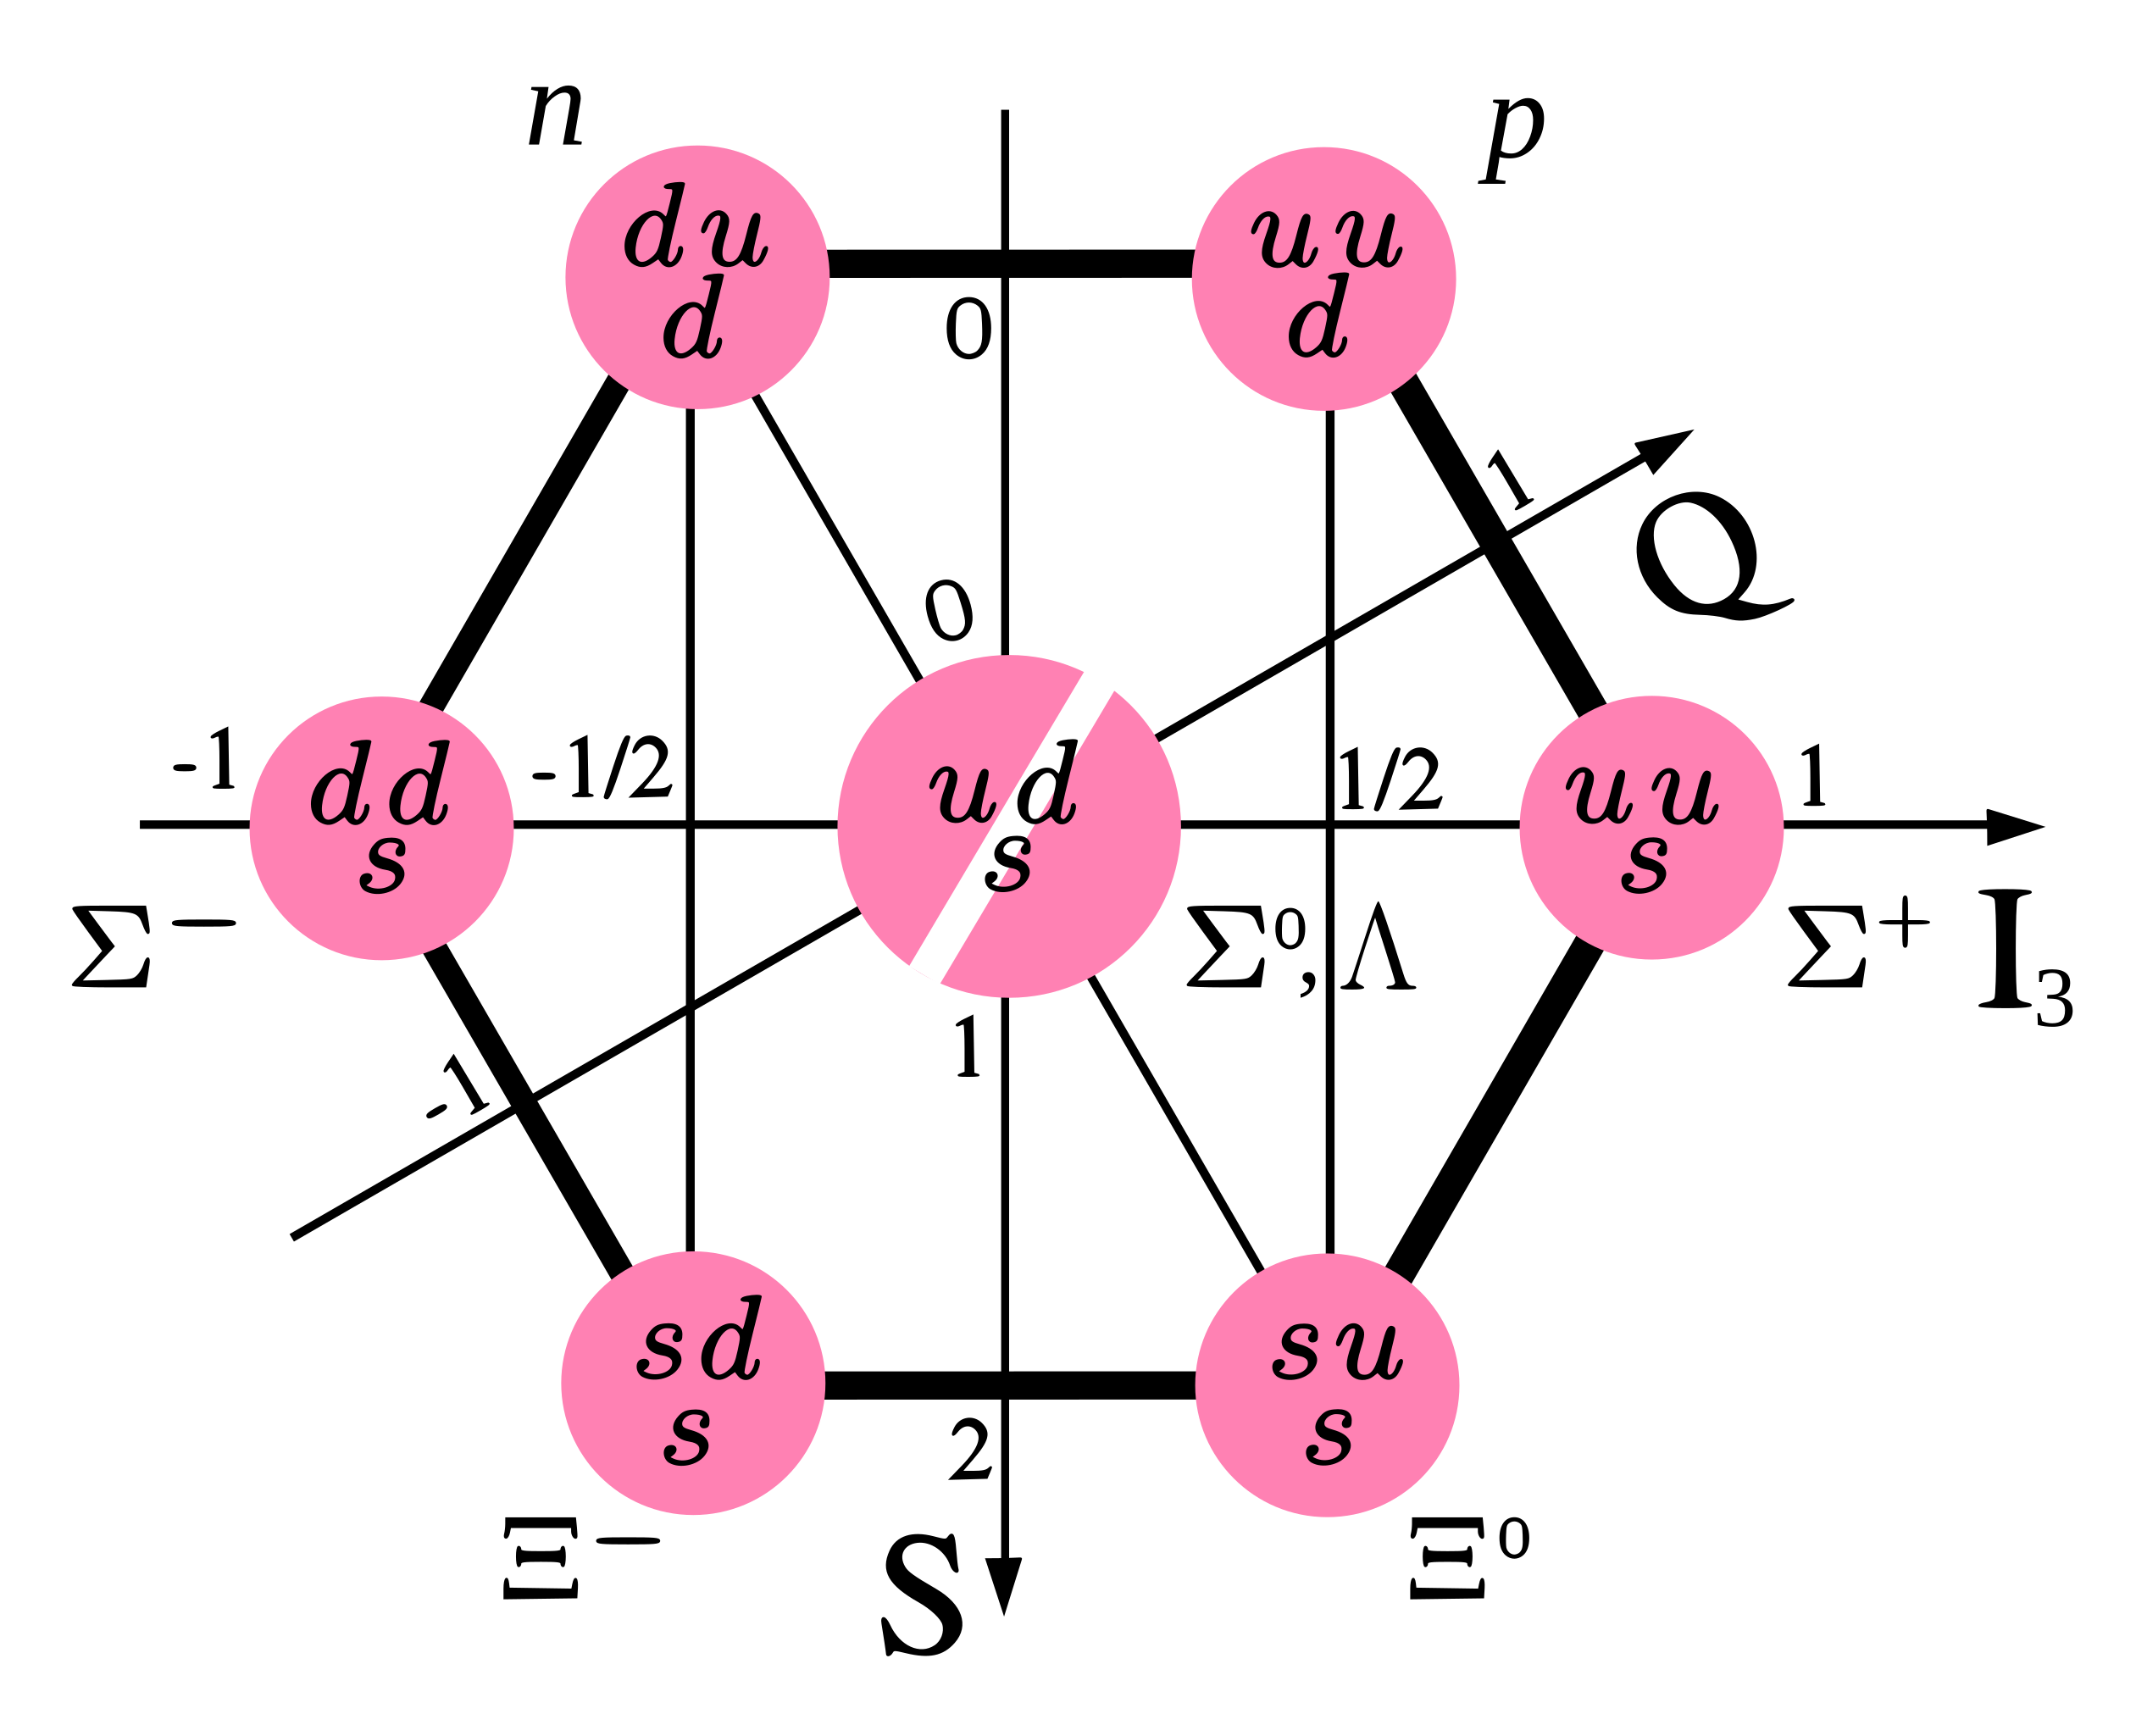
\includegraphics[width = 0.49\textwidth]{baryon-octet.png}
	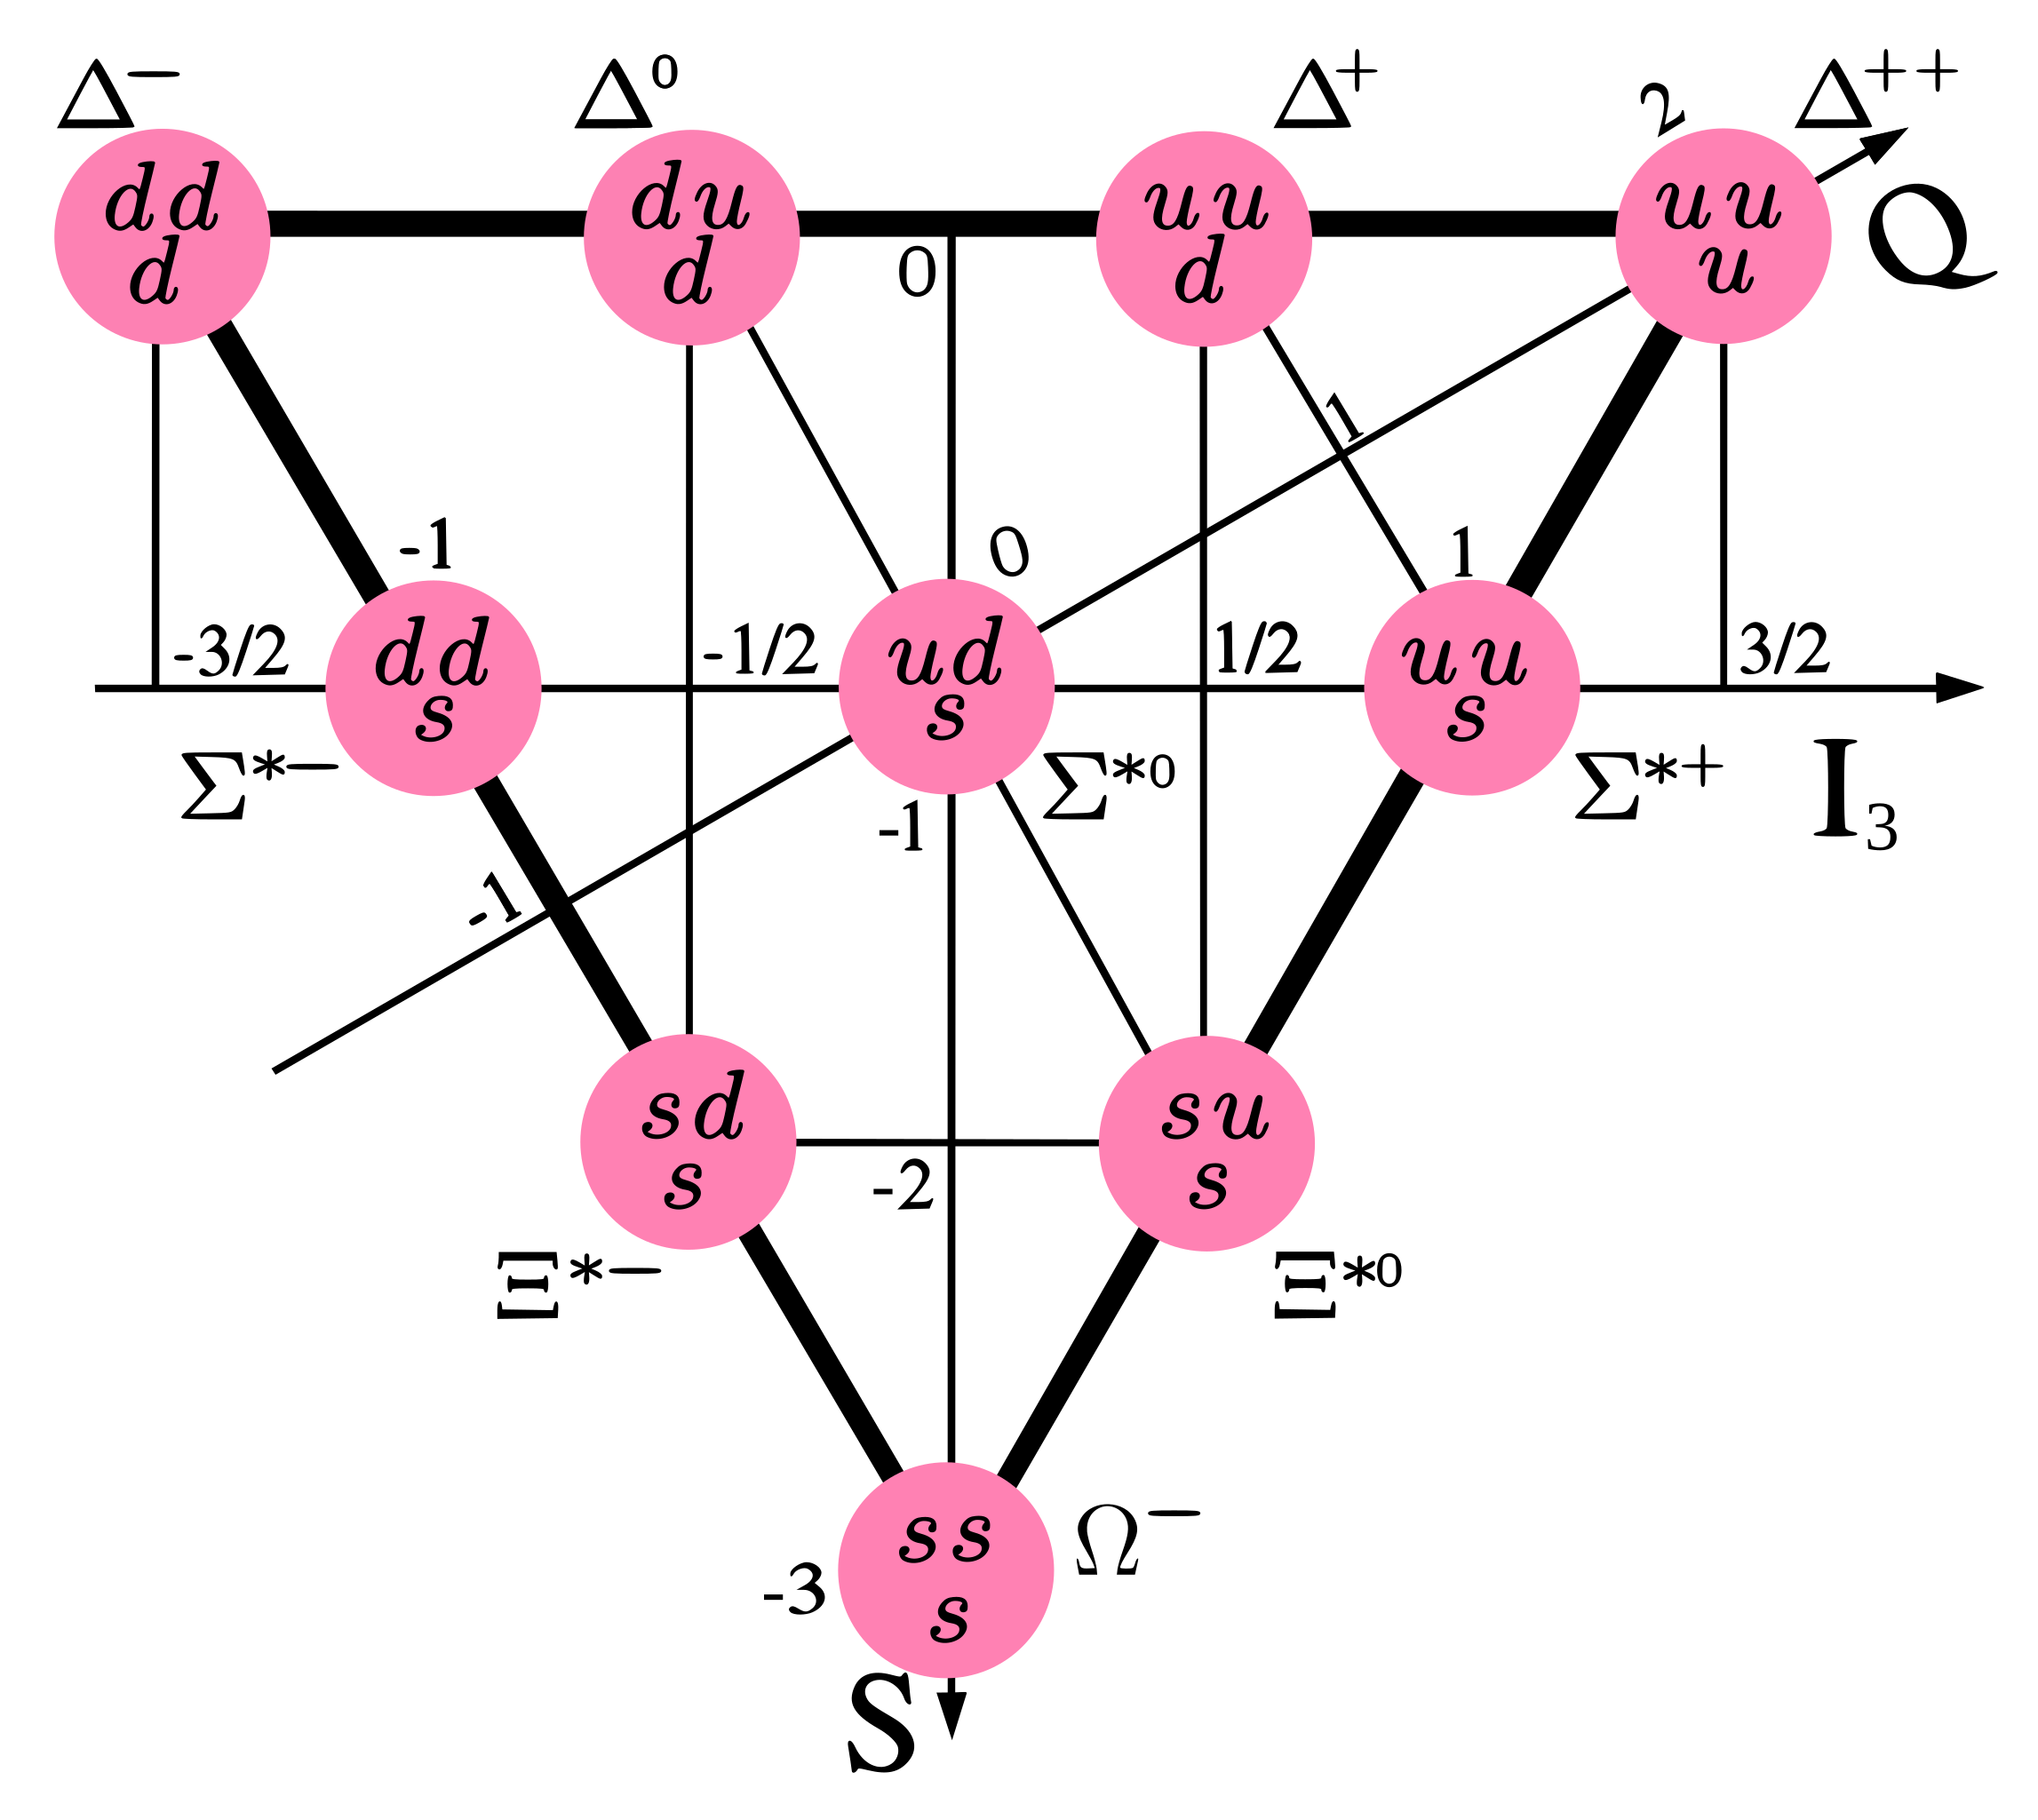
\includegraphics[width = 0.49\textwidth]{baryon-decuplet.png}
	\caption{Baryon octet ($ s = \frac{1}{2} $) and decuplet ($ s = \frac{3}{2} $).}
	\label{baryons}
\end{figure}
\begin{figure}
	\centering
	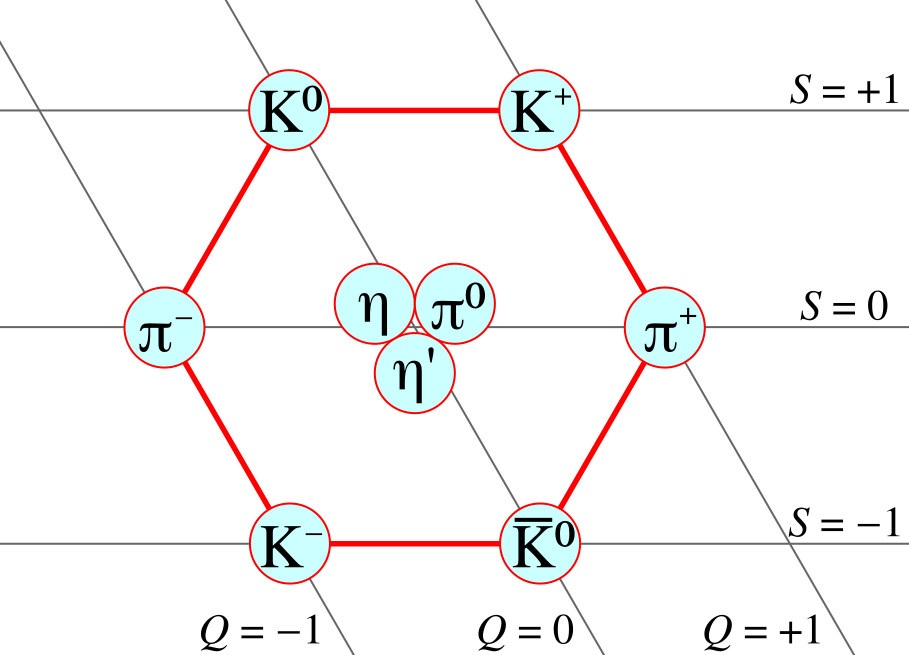
\includegraphics[width = 0.49\textwidth]{meson-nonet-1.png}
	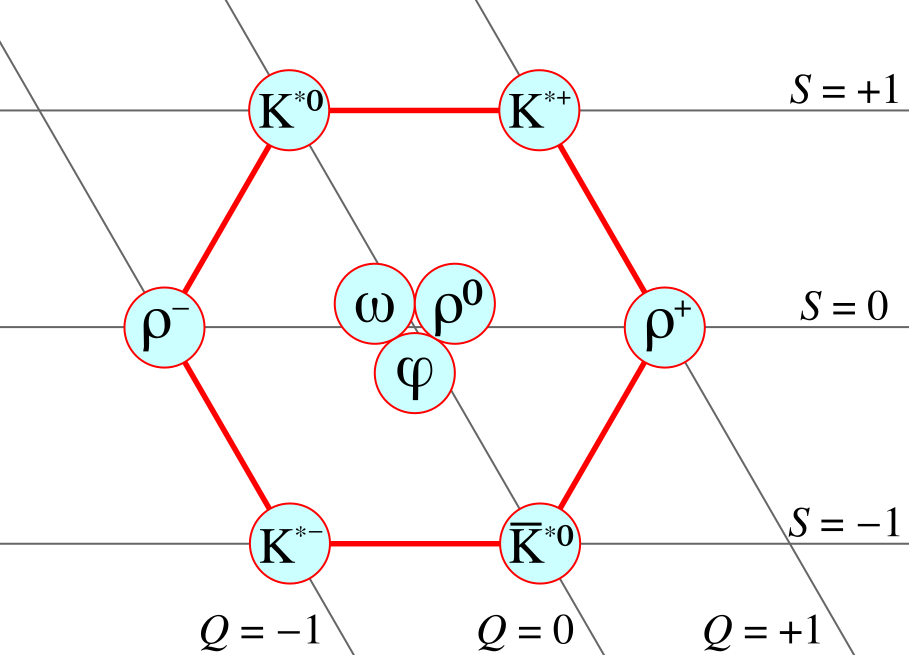
\includegraphics[width = 0.49\textwidth]{meson-nonet-2.png}
	\caption{Meson nonets ($ s = 0 $ and $ s = 1 $).}
	\label{mesons}
\end{figure}

\subsection{Colore}

Si può notare che il modello a quarks postula che dei quarks identici occupino lo stesso stato quantistico all'interno di alcuni barioni: ad esempio, nei barioni $ \Delta^{++}(uuu) $, $ \Delta^- (ddd) $ ed $ \Omega^-(sss) $ tre quarks identici si trovano tutti in uno stato con $ \ell = 0 $ e $ s = \frac{1}{2} $, risultando simmetricamente scambiabili tra loro. Per non violare il principio d'esclusione è dunque necessario introdurre un nuovo numero quantico, al fine di distinguere gli stati di questi quarks altrimenti identici: il \textit{colore}. I numero quantico di colore ha tre possibili valori: blu ($ \mathsf{b} $), rosso ($ \mathsf{r} $) e verde ($ \mathsf{g} $), ai quali sono associati anti-blu ($ \bar{\mathsf{b}} $), anti-rosso ($ \bar{\mathsf{r}} $) ed anti-verde ($ \bar{\mathsf{g}} $) per gli antiquarks.\\
Una proprietà fondamentale del colore è che solo particelle incolori possono essere osservate: queste sono particelle in cui sono combinati colore e rispettivo anticolore (mesoni), oppure tutti e tre i colori in egual misura (barioni); le altre combinazioni non sono permesse. Questo è il motivo per cui non si osservano quark singoli: essi vengono istantaneamente confinati in adroni.\\
Il colore, così come gli altri numeri quantici associati ai quarks (isospin, stanezza, charm, bottomness e topness) sono conservati dall'interazione forte, ma non da quella debole. Risulta quindi che la maggior parte degli adroni decade forte, con vite medie $ \tau \sim 10^{-23}\,\text{s} $; gli adroni con le masse più piccole per ciascun set di numeri quantici (adroni strani, adroni charm, etc.), invece, non possono decadere forte poiché non ci sono particelle più leggere con gli stessi numeri quantici: di conseguenza, hanno vite medie più lunghe poiché decadono tramite interazione debole ($ \tau \sim 10^{-7} - 10^{-13}\,\text{s} $) o elettromagnetica ($ \tau \sim 10^{-16} - 10^{-21}\,\text{s} $).

\subsubsection{Cromodinamica Quantistica}

La natura della forza forte è legata al colore: si parla infatti di \textit{carica di colore}. Il force carrier del color field (o strong field) è il \textit{gluone}, un bosone massless e con spin 1.\\
Essendo mediatori dell'interazione tra quarks, i gluoni devono essere portatori di due colori, e nello specifico di un colore e di un anti-colore: ad esempio, la reazione $ u_{\mathsf{r}} + d_{\mathsf{b}} \rightarrow u_{\mathsf{b}} + d_{\mathsf{r}} $ è mediata da un gluone $ \mathsf{r}\bar{\mathsf{b}} $ emesso dal quark up ed assorbito dal quark down. Le possibili combinazioni colore - anti-colore sono 9, ma quelle colorless $ \mathsf{b}\bar{\mathsf{b}} $, $ \mathsf{r}\bar{\mathsf{r}} $ e $ \mathsf{g}\bar{\mathsf{g}} $ vanno opportunamente combinate secondo le regole di simmetria del color field:
\begin{equation*}
	\frac{1}{\sqrt{2}} \left( \mathsf{r}\bar{\mathsf{r}} - \mathsf{g}\bar{\mathsf{g}} \right)
	\qquad
	\frac{1}{\sqrt{6}} \left( \mathsf{r}\bar{\mathsf{r}} + \mathsf{g}\bar{\mathsf{g}} - 2\mathsf{b}\bar{\mathsf{b}} \right)
	\qquad
	\frac{1}{\sqrt{3}} \left( \mathsf{r}\bar{\mathsf{r}} + \mathsf{b}\bar{\mathsf{b}} + \mathsf{g}\bar{\mathsf{g}} \right)
\end{equation*}
Soltanto le prime due di queste tre combinazioni possono effettivamente trasmettere colore, dunque in totale ci sono 8 gluoni.\\
I quarks all'interno degli adroni sono legati dal color field scambiandosi gluoni, dunque cambiano continuamente colore, ma sempre preservando la neutralità overall dell'adrone. I quarks non possono esistere in maniera individuale poiché la color force cresce d'intensità all'aumentare della distanza: man mano che due quarks si allontanano tra loro, l'energia d'interazione aumenta fino al punto che è sufficiente a creare una nuova coppia quark-antiquark, formando quindi due particelle overall sempre colorless. Si vede dunque che se ad un adrone viene data sufficiente energia, ad esempio da scattering ad alte energie, non si riesce mai ad estrarre un singolo quark da esso, ma il risultato sarà sempre la produzione di altri adroni (tendenzialmente mesoni).\\
Le interazioni tra quarks danno luogo alle forze nucleari: sebbene i protoni nel nucleo si respingono tra loro per via dell'interazione elettromagnetica, l'interazione forte tra i rispettivi quark ha un'intensità maggiore, dunque i due nucleoni rimangono legati.










